\chapter{Autonomic and Self-Organizing Systems: A Review} % Write in your own chapter title
\label{Chapter_related}
\lhead{Chapter \ref{Chapter_related}. \emph{Autonomic and Self-Organizing Systems: A Review}} % Write in your own chapter title to set the page header

This chapter presents the known approaches for autonomic computing and self-organizing systems and motivates the need for developing a self-organizing architecture for the autonomic management of cloud resources, including the advantages that such an architecture would provide. The chapter also introduces prior work in the area of simulation systems for clouds and provides motivation why the simulation framework used in this thesis was selected.

\section{Reasons for Self-organizing Architecture}

Since the introduction of autonomic systems by IBM \cite{IBM:acblueprint}, autonomic systems have been developed using the Monitor, Analyze, Plan, Execute (MAPE) loop. Figure \ref{fig:MAPELoop-IBM} shows the loop as described by IBM. The resource under control, which can be as simple as a single server or as complex as a cluster of servers, is constantly being monitored to determine changes in its state. This monitoring can be either periodic measurements of certain values in the system, like CPU utilization or response time, or alarm-based when certain conditions are breached and an alarm is raised. Once the measured or alarm data is obtained by the monitor function, the data is passed on to the analyze function which uses its internal logic and rules in order to analyze the data and to determine if the system is exhibiting any problems. If a problem is discovered, the problem information is sent to the plan function whose role is to determine an appropriate response to fix the existing problem or problems. The plan function creates an execution plan which will fix the problem and bring the controlled resource back into compliance. The execution plan is then delivered to the execution function which puts the plan into execution by making modifications to the resource and to the resource's environment.

\begin{figure}
	\centering
		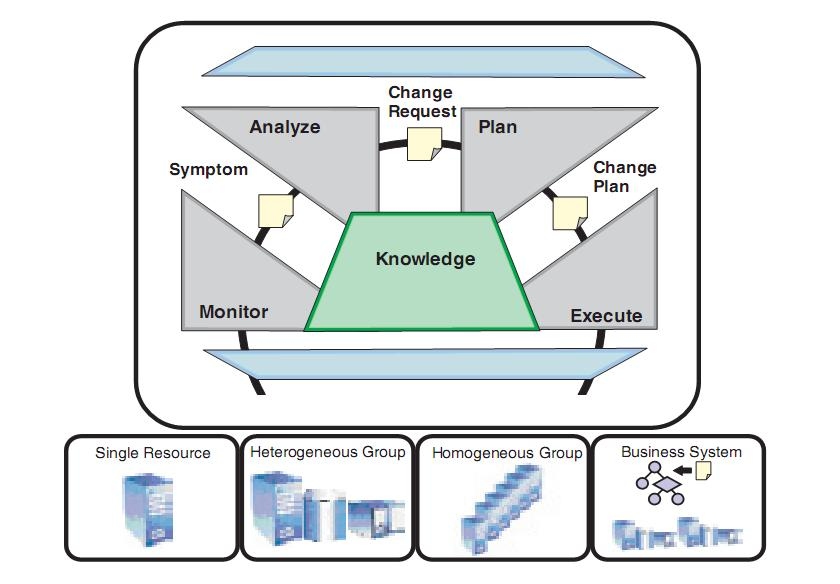
\includegraphics[width=14.6 cm]{MAPELoop-IBM.jpg}
		\caption{MAPE Loop}
	\label{fig:MAPELoop-IBM}
\end{figure}

In order to illustrate the autonomic system approach, consider a cloud of servers. The goal of the autonomic system is to maintain a good utilization of the server resources, while at the same time guaranteeing a certain level for the cloud's response time. For such a case, the autonomic control loop would measure all the servers' response times and CPU usage. If the response time becomes too high, as determined by the analyze function, the plan function calculates how many new servers to add to the cloud. Once the number of new servers is determined, the execute function is responsible for bringing those servers online by starting them and adding them to the cloud. If the CPU usage of the servers in the cloud decreases too much however, the plan function calculates how many servers to remove from the cloud. It is then the responsibility of the execute function to stop the correct servers, remove them from the cloud and free any other resources used by the servers.

Two main approaches have been taken in research in order to build autonomic systems. These approaches are presented in more detail in the following sections. The first approach considers the entire system under control as a single unit and attempts to add a global control loop which controls the entire system. In the above example, such a system would gather data from all the servers and use some form of mathematical approach like an averaging of the measured data in order to estimate the state of the entire cloud. Based on this average, the system would then determine any breach of Service Level Agreement (SLA) and create a plan if a breach exists. This approach has a number of assumptions on how the cloud is formed and how the cloud behaves. First of all, the autonomic control system assumes all the servers in the cloud are exactly the same. If the cloud was heterogeneous, then it would not be possible to average the measured data to obtain a global view of the cloud - unless a more complex procedure is used where the analyze function also knows ahead of the time the relative power of all the servers. Second of all, the system not only assumes that all servers are the same, but also behave the same, and, in addition, that client requests are balanced appropriately across all servers. If this was not the case, it would be possible to have, for example, two types of requests A and B, where A type requests are much more computationally intensive than B, and where all the A requests go to Server 1 and B requests to Server 2. Such a case could lead to an undesirable situation where the response time of Server 1 is above the desired SLA, but the average between Server 1 and Server 2 is below the desired SLA.

The second approach views the system under control as a composition of smaller subsystems (servers in the example given above) which are to be controlled. Through the control of each of these subsystems, a desired global SLA level can be reached. In the above example, each of the servers would have its own control loop responsible only for that server and which is ensuring that the server maintains a response time bellow the required SLA. Such an approach allows for heterogeneous resources to be part of the same cloud. It also allows for mixed clouds which can contain virtualized and non-virtualized servers running together. Furthermore, requests do not need to be balanced across servers; as long as each server correctly maintains its own SLA, even if the cloud encounters a case similar to the previous example where all request of type A come to one server and all requests of type B reach another server, the system will maintain a good SLA across all servers in the cloud. An extra advantage of this approach is that it scales very well even with a very high number of subcomponents (servers). For the centralized approach, if the number of servers increases too much, the central controller starts exhibiting load and latency issues as well. With a decentralized approach, the cloud can theoretically grow forever without suffering degradation due to the control plane. The problem with decentralized systems is that they are more complicated to design, deploy and manage.

There are other approaches used in literature which are somewhere between a fully centralized and a fully decentralized approach. For example, hierarchical controllers may have subcontrollers that take local decisions under the supervision of a parent controller. Such systems will exhibit some of the drawbacks of fully centralized systems but without all the design and deployment problems of fully centralized systems.

One approach which matches well to decentralized systems is the approach of Self-organizing systems, as Self-organizing systems are systems in which a desired state is reached without the use of any central authority or plan. Self-organizing Systems can achieve high-level goals via the interaction and communication between the components and without the need for a global controller which manages each and all of the subcomponents of the system. From these interactions and communications an emergent system appears which can exhibit self-optimizing features as required by autonomic computing. This approach is the one taken in this thesis due to the advantages that it offers compared to a global controller.

\section{Related Work}

Autonomic computing has become a very important field in research and industry due to the complexity of the IT infrastructure. Autonomic computing is also one of the fundamental technologies required for cloud computing and management of virtualized resources. All autonomic research is based on the MAPE loop in one form or another. This, however, did not prevent a diversity of approaches to be taken. Multiple architectures have been proposed, as well as various control techniques from machine learning to control theory. This section will be composed of related work in autonomic system architectures, various approaches for the MAPE loop components, self-organizing systems, as well as in real-time collaborative systems.

\subsection{Autonomic System Architectures}

All autonomic system architectures are based on the initial proposal of the MAPE loop made by IBM, also sometimes known as a MAPE-K loop to include the knowledge portion of the system. However, the use of the MAPE-K loop as a starting point did not hinder a variety of architectures from being proposed in research. The autonomic system architectures which can be found in literature can be split into three main types: decentralized architectures, hierarchical architectures and centralized architectures.

\subsubsection{Centralized Architectures}

Centralized architectures have a common characteristic in that the entire autonomic system - excluding sensors which can run on the measured entity - is running on a single machine which is responsible for running the entire MAPE-K loop and managing all the required resources. Such an approach can be found in the work done at Montana State University \cite{related:architecture:autonomicelement} where the autonomic architecture is developed as an Autonomic Element. The autonomic element is seen in this paper as the base building block for an autonomic system. An autonomic element is composed of two parts: the manager and the managed element. In their paper, the manager is described as a multi-threaded daemon, with each of the four MAPE functions, as well as the effectors and sensors, running in their own threads. Message passing is done via queues and synchronization is obtained via semaphores. Figure \ref{fig:centralizedarchi} shows a typical centralized architecture for three servers. All server data is measured by one controller, which performs the MAPE process and then takes control actions on the servers.

\begin{figure}
	\centering
		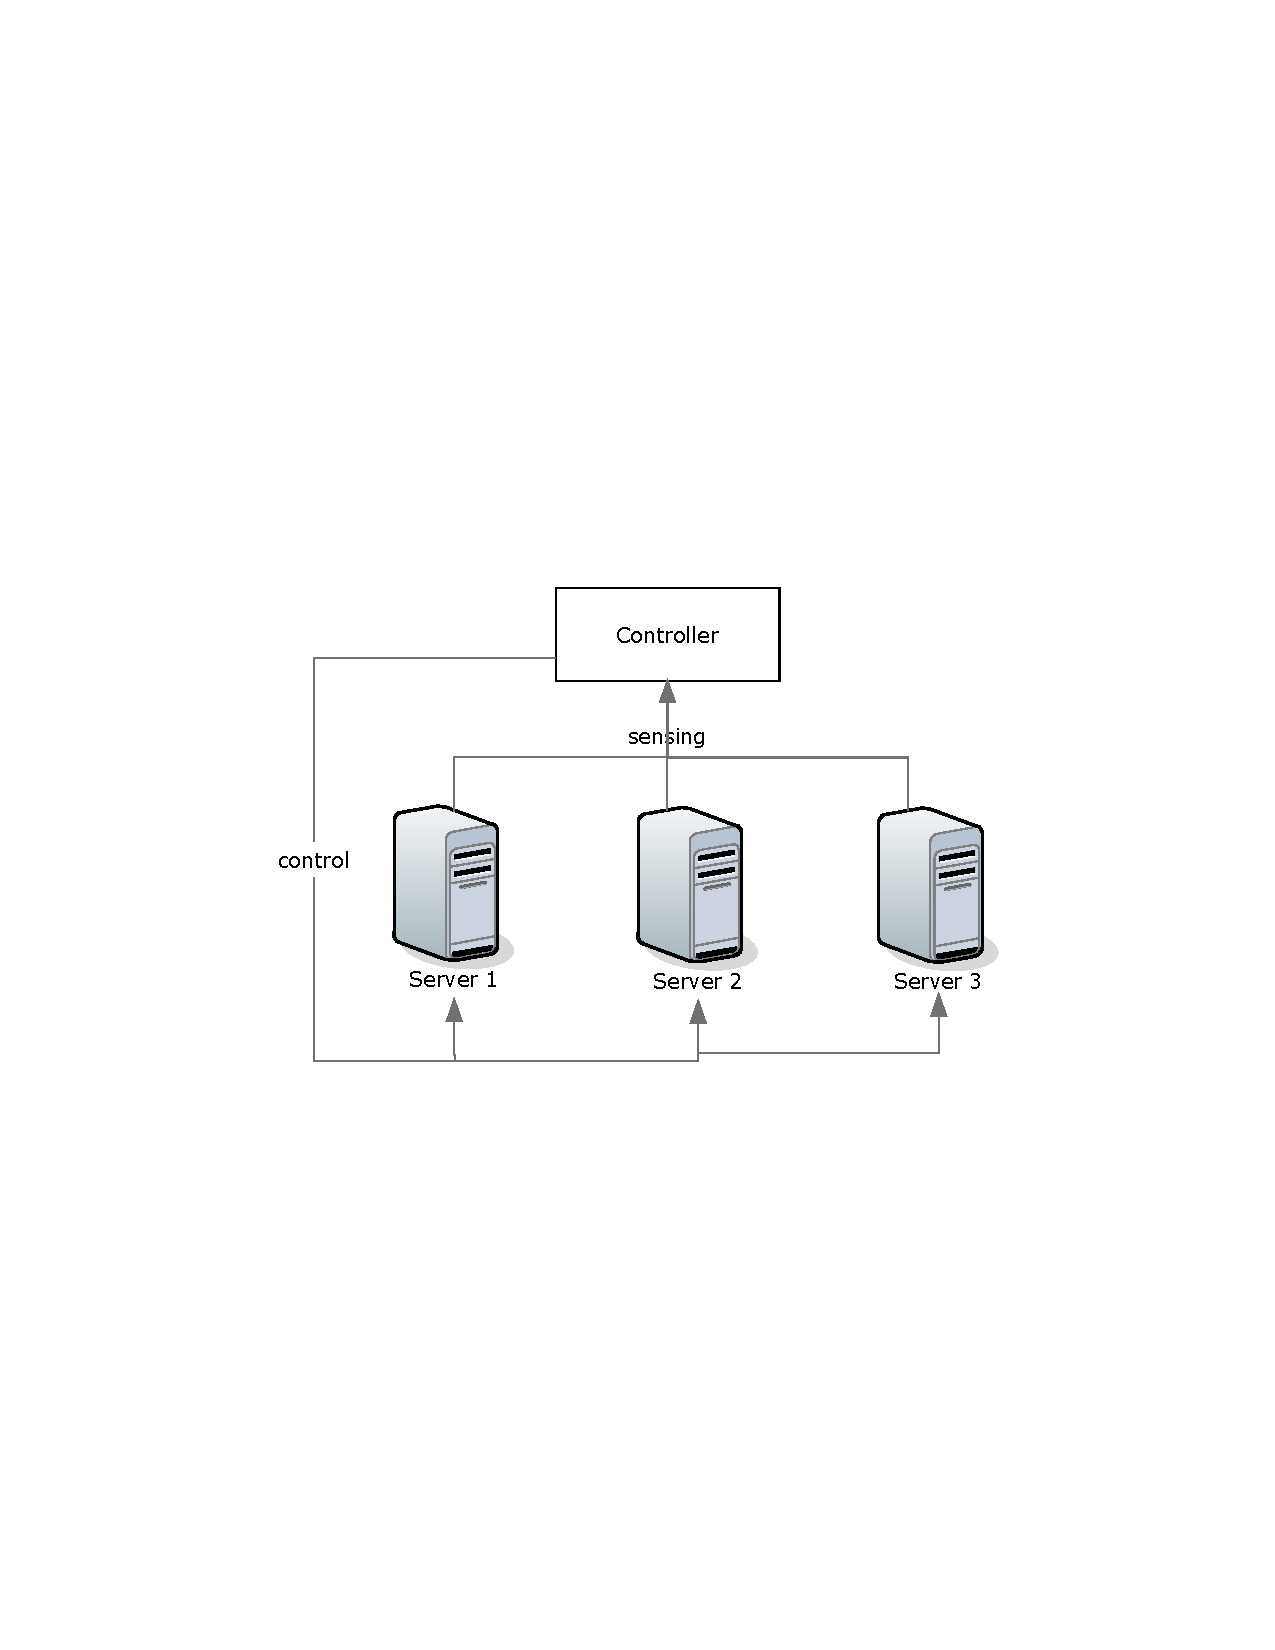
\includegraphics[width=0.75\linewidth]{ThesisRelatedArchiCentralized}
	\caption{Centralized Autonomic System Architecture}
	\label{fig:centralizedarchi}
\end{figure}

The architecture uses sensors to obtain data about the managed element and the environment, and defines two separate sensors for each autonomic element - one for internal data from the managed element and an external one for data from the environment. Similarly there are two effectors: one which passes required changes to the external environment and one which modifies the managed element internally. Furthermore, the architecture defines a ``data atom'' as the basic message that is passed throughout the system. Each atom is an XML data structure that contains version, priority, type and meta-data as well as the base data for the event. Furthermore, multiple atoms can be chained together to form a single atom if required by some common relation.

Since the architecture for an autonomic element uses separate threads for processing, care must be taken to ensure that the system performs correctly asynchronously and that there are no deadlocks in the system. In order to ensure the above, the authors of \cite{related:architecture:autonomicelement} propose the use of a priority queue for message passing. As data atoms are sent from one component to another, the atoms are stored in a queue based on their given priorities. The components then pop the respective atoms, process them, and either send them forward to the next component, create new atoms to be sent, or send the atoms to an empty data sink to be destroyed. In order to prevent deadlocks and starvation, the authors also use an extra object named a ``locker'', which is similar to a semaphore. A locker is placed between each two adjacent components and its role is to pass atoms between components. A locker receives an atom from a sending component, and notifies the receiving component that it has a new atom available for processing. Since polling is not used, it prevents synchronization and deadlock issues. Lockers are unidirectional, making it impossible to send data back to a previous component for processing, thus resulting in a sequential processing of data. In order to provide rapid response for sensors and effectors, the architecture uses data streams, which are one-way communication channels where one component writes data, and another reads the data in an atomic way. The system also uses a repository to store both processed atoms that are needed later, as well as policy rules. This repository acts as the knowledge base in the MAPE loop.

The above architecture has a number of problems which make it hard to use in most cases. First of all, the autonomic element architecture executes its entire process on a single machine. This causes problems, which apply to all centralized approaches, in cases where the managed element is a large structure, like a cloud, formed from hundreds of resources. A centralized approach will scale poorly as the number of resources which are monitored and managed increases. Furthermore, in the case of geographically distributed resources, the sensor data from the managed resources would have to travel through the internet to the manager, which can add large delays to processing the data and taking corrective actions. Finally, the architecture forces an autonomic element to have two sensors - one external and one internal, as well as two effectors. However there are cases were data comes from a varied number of sources, possibly each with its own data sample period, and where splitting the data inputs into more than two sensors is desired. Because of the above factors, the autonomic element architecture is restrictive in terms of the kind of autonomic system which can be developed and deployed.

Centralized architectures are also used by some systems developed in industry like IBM's Tivoli Intelligent Orchestrator (TIO) \cite{product:tio} and Sun N1 Service Provisioning System (SPS) \cite{product:n1}. TIO is capable of analyzing the CPU utilization of servers in a cluster and based on utilization over time, along with future predictions, decide if servers must be added or removed. Once a decision is reached, TIO deploys additional servers by finding available servers and, based on predefined workflows, provisions those servers and adds them to the cluster. A number of issues exist with the TIO platform. First of all, TIO assumes that all the servers in a cluster or resource pool are homogeneous in hardware and have the same behavior. This is rarely the case in data centers and even more so in clouds, where the deployment location could vary. Furthermore, even two computers with the same software/hardware will exhibit slightly different behavior. Second of all, TIO can not monitor multiple metrics, and provide multiple provisioning decisions to the same cluster. Only the CPU is monitored and only add/remove server actions are supported in the autonomic mode. Third of all, TIO is designed as a monolithic piece of software, making it hard to extend in order to add extra intelligent behavior. Unlike TIO which manages clusters of servers, N1 automates the deployment and configuration of web applications, thus providing the self-configuration characteristic of autonomic computing. Similarly to TIO, SPS is capable of provisioning operating system clones and applications in order to quickly configure a new server.

\subsubsection{Hierarchical Architectures}

Hierarchical architectures improve on centralized architectures by using multiple MAPE-K loops which are organized in a pyramid, with the low level control loops managing fine grained resources, while the high level control loops are responsible for the state of the entire system. Figure \ref{fig:hierarchicalarchi} shows a typical two-layer hierarchical architecture for three servers. Each of the servers has its own control loop and all the low-level control loops have a second layer which manages their parameters.

In \cite{Kramer:hierarch}, the authors propose a three layer architecture formed from bottom to top from: component control, change management and goal management. At the lowest level, the component control layer is concerned with short time scale operations and its goal is to modify the operating parameters of the component under management. At the change management level the system responds to changes in state reported from the lower level. This layer is reactive in that in response to a change in the lower level, it creates a plan to improve or maintain the execution of the system. This layer can, for example, add new components or modify existing components to maintain SLAs. Finally, the goal management layer is responsible for long timescale operations. It takes the state of the system and long ranging goals and produces plans which reach those goals. For example, this layer would be responsible to find available servers which should be deployed in order to maintain a required SLA, or how to migrate servers to maintain a desired redundancy rate after a server's failure. It should be noted that the author's architecture is based on Gat's model for robot architectures \cite{gat:robots}. 

\begin{figure}
	\centering
		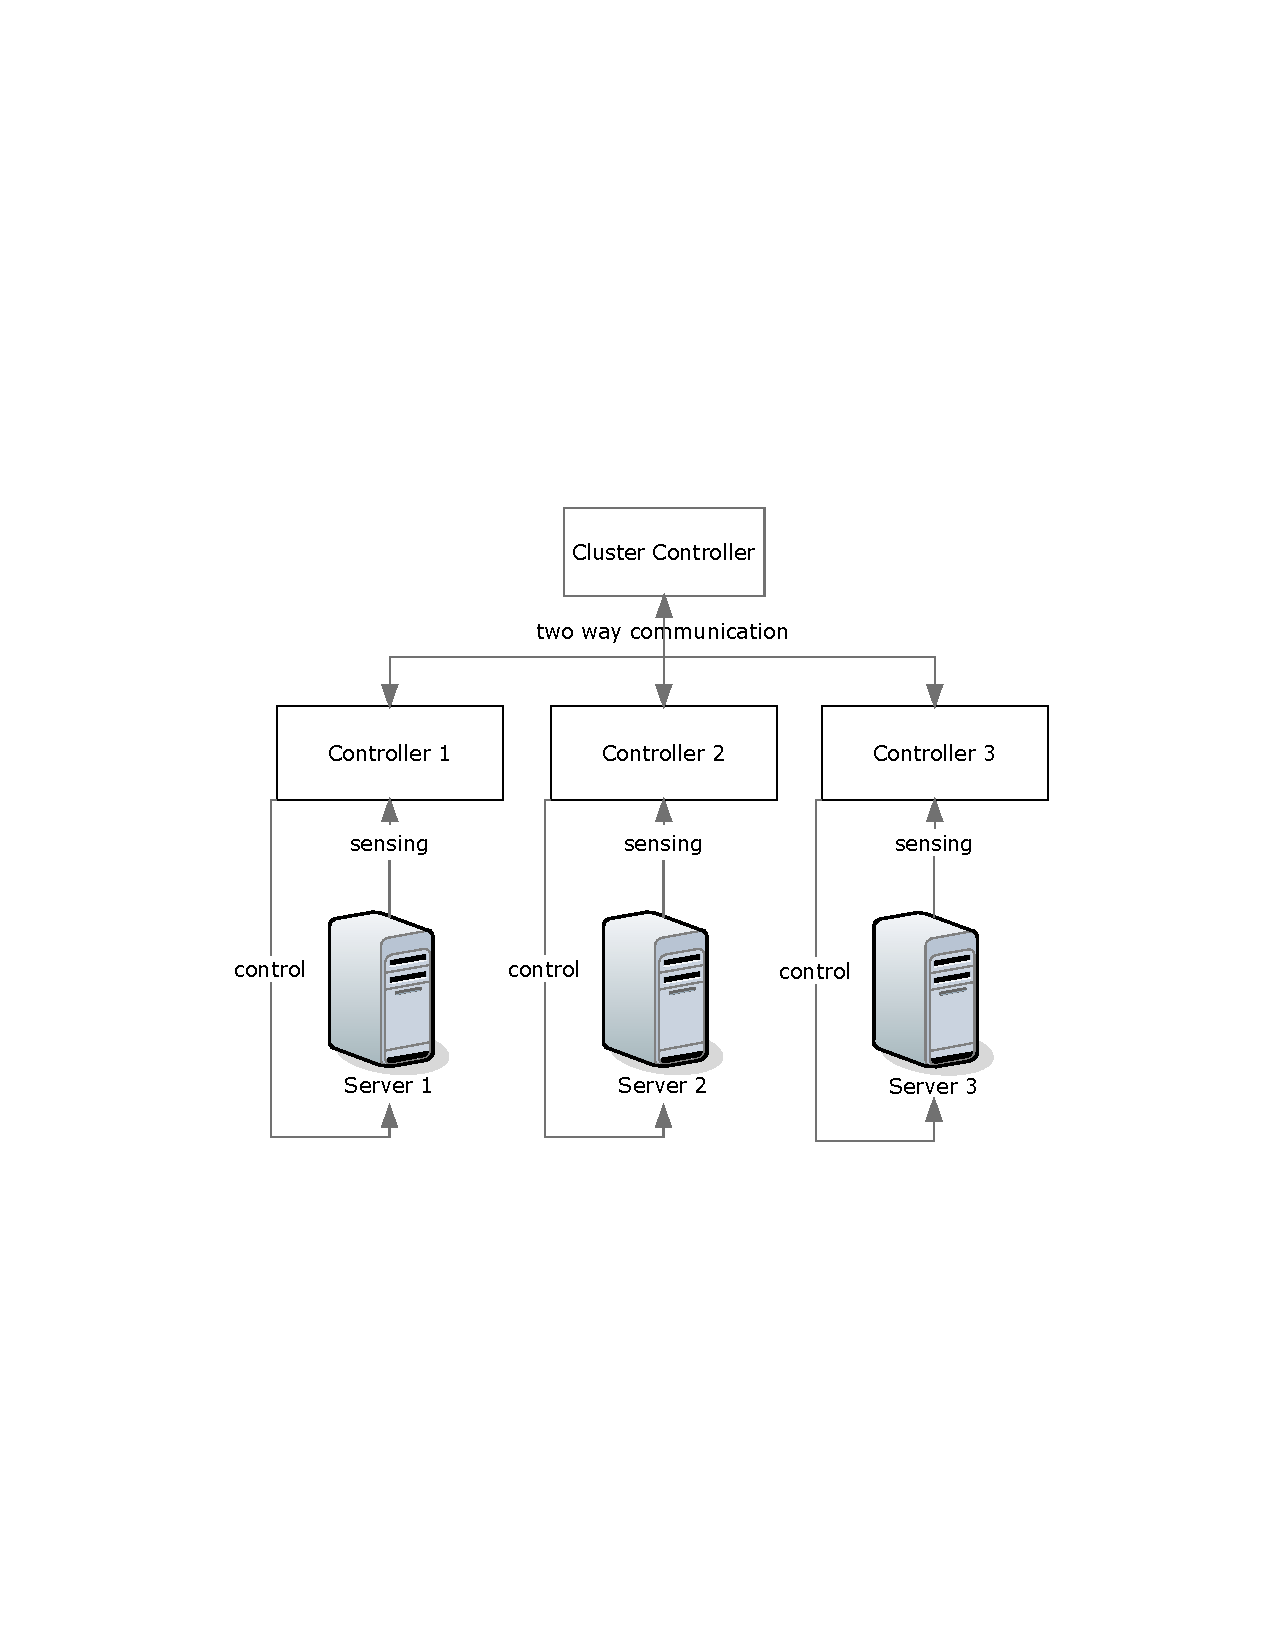
\includegraphics[width=0.75\linewidth]{ThesisRelatedArchiHierarch}
	\caption{Hierarchical Autonomic System Architecture}
	\label{fig:hierarchicalarchi}
\end{figure}

Similarly, in \cite{related:architecture:hierarch2}, the authors develop a three layer architecture where the system manages from bottom to top: the component, the application and the system. Similarly to the work in \cite{Kramer:hierarch} the component level manages a single component and takes actions that span a short time. This could be for example a web server which modifies its buffer pool size or thread pool size. By itself, this is not sufficient to manage the SLA of the system and the component level also can not set its own QoS targets. The middle level controller which is the application controller, manages the performance of the entire system by setting QoS parameters for the lower level controllers and taking over when the low level controllers can not reach the required QoS. Such an action could be to redistribute incoming requests to ensure that some servers are not overloaded. The highest layer controller - the provisioning controller - is responsible for rearranging the system when it can not meet its QoS without structural changes. Such changes can include adding or removing servers to/from the cluster in order to maintain the QoS attributes while also ensuring optimal utilization of resources.

While hierarchical architectures improve on centralized architectures by separating the control concern into multiple levels, where long running self-managing decisions can run at a higher level, while short timeframe decisions can be made close to the component to be changed, some of the issues with centralized architectures still remain. First of all, the use of high level control loops still forces an assumption that the systems components are homogeneous. If the components were to be heterogeneous, then then high level control loops would need to make use of complex models to represent the variation in power of the various components. Second of all, high level control loops would still face scaling problems as the number of components to be managed grows.

\subsubsection{Decentralized Architectures}
\label{sect:decentralized}

Decentralized architectures make use of no global controller and base themselves on the interaction between components to reach a self-managing state. Figure \ref{fig:decentrarchi} shows a typical decentralized architecture for three servers. Each of the servers has its own control loop and the autonomic behaviour is obtained through the communications between the controllers of the servers. Note that not all servers have to communicate with all other servers.

\begin{figure}
	\centering
		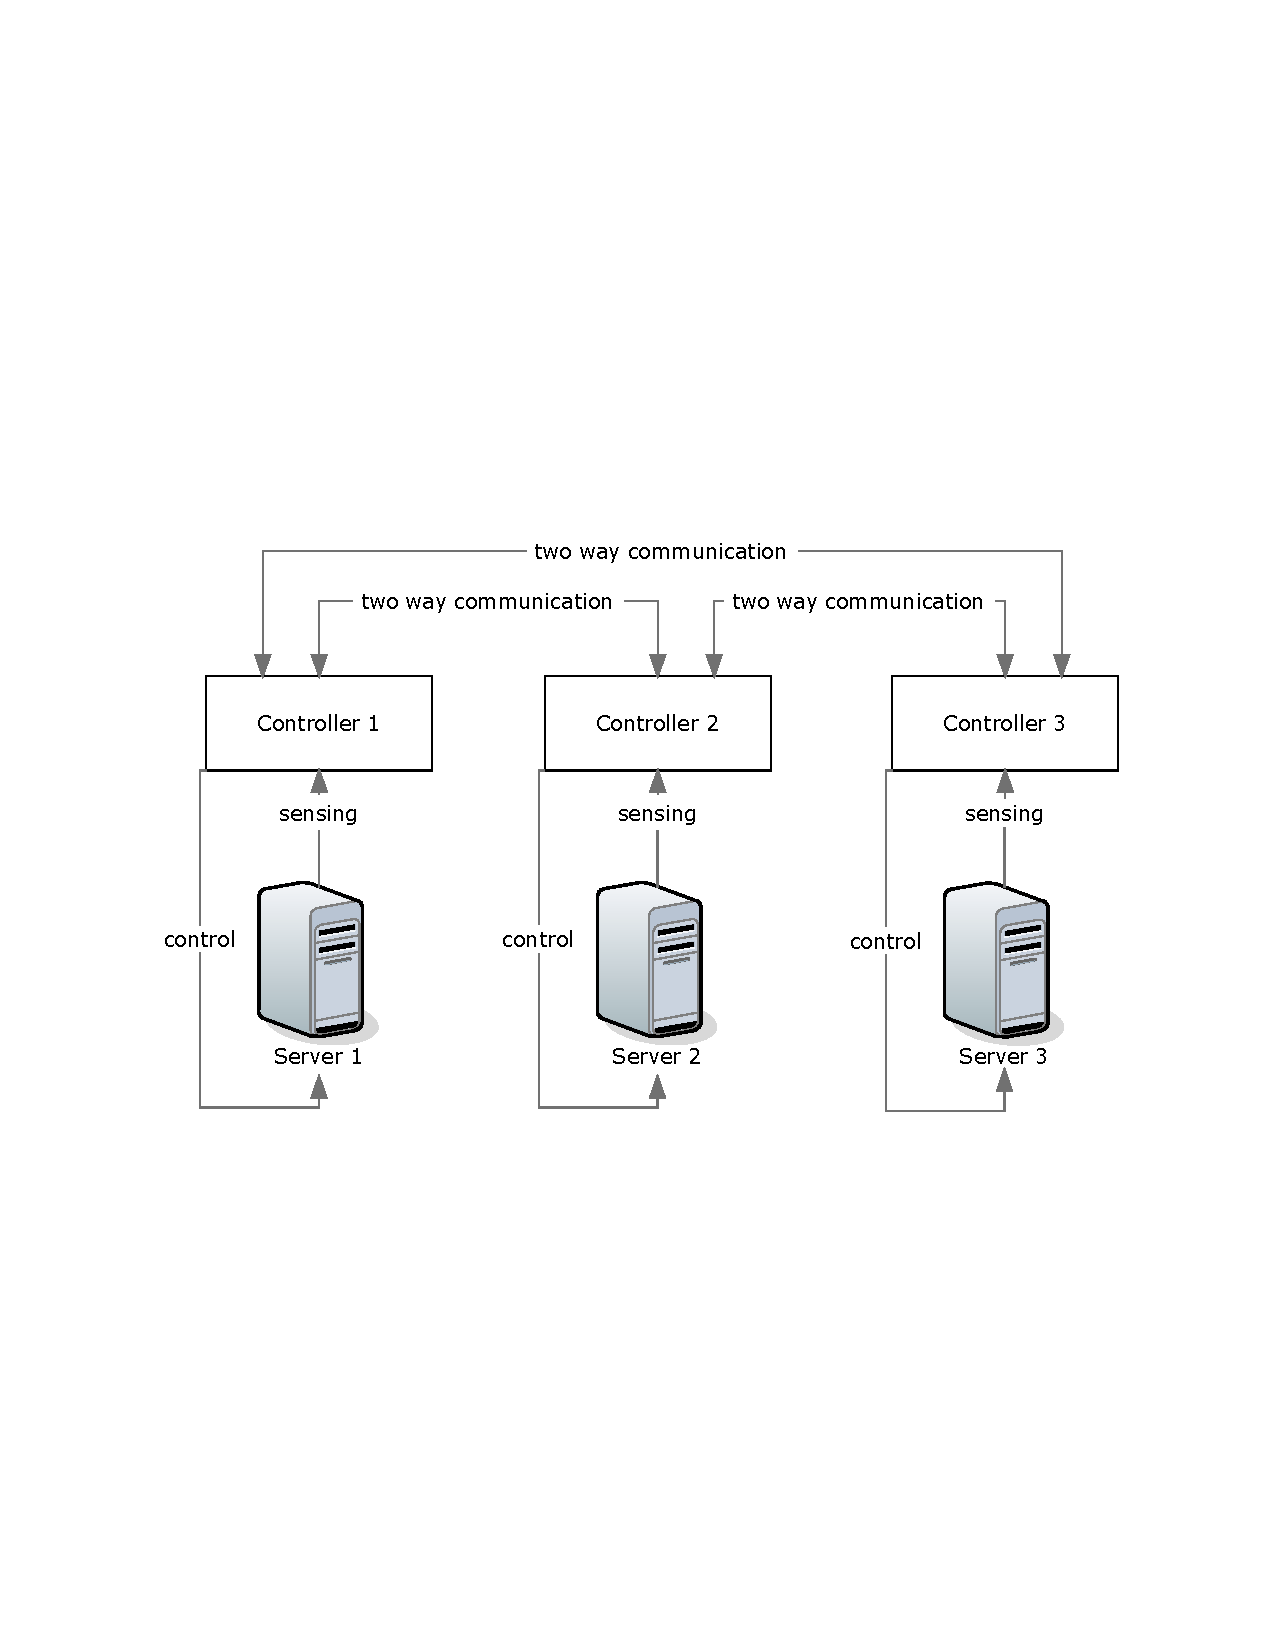
\includegraphics[width=0.75\linewidth]{ThesisRelatedArchiDecentralized}
	\caption{Decentralized Autonomic System Architecture}
	\label{fig:decentrarchi}
\end{figure}

Approaches to create such system range from biologically inspired architectures to self-organizing systems. Such an approach to build autonomic systems is that of a self-managing peer-to-peer architecture, as described in \cite{related:architecture:selfmanagep2p}. In this approach each element of the managed resource has its own management logic, and the overall Quality of Service (QoS) is achieved through peer-to-peer negotiation between the elements. While the architecture does distribute the management function across various elements, the architecture is not fully peer-to-peer, the authors choosing a hybrid approach. The top level of the QoS is reached through peer-to-peer negotiations, the lower level state is reached through hierarchical control. The described approach is meant for ``the autonomic management of heterogeneous networks and services'' \cite{related:architecture:selfmanagep2p}, but it can also be extended to other autonomic systems.

Another approach for developing decentralized autonomic systems is that of using biologically inspired architectures. In recent years, biologically inspired algorithms, like the Ant algorithm \cite{antalgorithm} for best route discovery in a network, have been investigated and developed. In \cite{related:architecture:selflet}, the authors propose an approach which is closer to biological models than to IBM's vision for autonomic systems. Instead of looking at an autonomic systems as a component that controls another resource, the authors design an autonomic system as a system that is able to change its internal behavior and its external interactions with other components, but is unable to modify external components. In order to reach this design, the authors create a ``SelfLet'' which is a self sufficient component, able to interact with other SelfLets in order to reach the high-level goals of the system. Each SelfLet has one or more behaviors, goals and actions. A goal represents a high-level objective, which can be achieved by executing some behaviors. Behaviors are performed by executing a set of local or remote actions. Similarly to the peer-to-peer architecture, SelfLets also have a negotiator manager, which they use in order to negotiate with other SelfLets a way to reach the goals.

Ant algorithms have also been investigated in autonomic systems. In \cite{statmechcomplexnetwork} the authors present an ant algorithm to decide where to place services in a cluster. Ants are created and sent in the datacenter to find available servers to use. As the ants traverse the servers in the cluster, they select servers where to deploy the service by examining each servers local state. Similarly, in \cite{messor:loadbalaneants} the authors use ant algorithm to determine load conditions and move jobs between servers in order to achieve load balancing in a data center.

In \cite{decentralized1} the authors use an approach similar to a peer-to-peer architecture. Each autonomic manager which comes online, for example for a new server starting, joins an autonomic management neighbourhood and exchanges messages periodically with members of the neighbourhood in order to determine the state of the system. Based on the information exchanged between autonomic managers, the autonomic managers can then make decisions on how to take actions to optimize the system. The authors apply the architecture to the grid problem of determining where to run various jobs in a grid while maintaining good performance for the various jobs running concurrently. In order to determine where to run the jobs, the system uses a neighbourhood of autonomic managers which decide the machines where jobs should be run, and, once started, monitor the jobs under their control to know the performance of the system. The managers also exchange information regarding the machines where jobs are being run and the performance of the respective jobs.

The decentralized approach has benefits in terms of scalability with respect to large systems, can be used for heterogeneous clouds and also works very well in systems where components can join and leave the system. As such, for the geographically distributed cloud presented in this thesis, the best approach is a self-organizing systems where each server manages itself and interacts with other servers in order to obtain a global optimal state for the entire cloud.

\subsection{Autonomic System Approaches}

In terms of approaches to creating the intelligent structure of an autonomic system, a variety of approaches also exists. Research into how to develop autonomic systems range from machine learning to control theory and include also policy based decision making, markovian models and economic models.

\subsubsection{Machine Learning}

Due to the fact that autonomic systems attempt to introduce intelligence into the management of the IT infrastructure, machine learning seems to be a very good approach to develop such systems. As such, machine learning methods have been widely used in research in order to create autonomic systems. 

In \cite{related:mldb} the authors use machine learning approaches in order to predict the performance of database queries using only information available before the queries execute. In order to achieve this goal, the authors examine five machine learning approaches: simple regression, clustering methods, principal component analysis, canonical correlation analysis and kernel canonical correlation analysis. The goal of the prediction was to try and compute, before a query is executed, and using only data about how the query is structured, and the query plan created by the database optimizer, multiple performance metrics such as CPU usage, memory usage, disk usage in order to be able to better predict resource contention in the database. Furthermore, the prediction had to perform well for both short running and long running queries, as well as for a database with a different schema than the trained database. The authors conclusions are that regression does a poor job of predicting the execution of SQL queries, in part because the regression algorithm ignored some of the query features when building the model. In terms of clustering, the authors conclude that for predicting both how long the query will take to execute and the performance characteristics of the query, they would need to run the clustering algorithm separately for each of the two datasets (execution time and performance characteristics). This approach would not find correlations between the two datasets. Principal Component Analsysis (PCA) has the same issue as clustering, as PCA can be applied only to a single multivariate dataset. Canonical Correlation Analysis (CCA) meets the authors goal of being able to find relations between pairs of multivariate datasets, however due to the fact that CCA uses an Euclidean dot product between the feature vectors of the two datasets to determine similarity the authors conclude that CCA is overly restrictive for the prediction of SQL query performance. Because of these restrictions, the authors use Kernel Canonical Correlation Analysis (KCCA) which is a generalization of CCA that uses kernel functions instead of Euclidean dot product for similarity measurement. The authors proceed to use KCCA in order to run experiments on a dataset constructed from a range of query types and obtain good results at predicting the performance metrics of the queries. 

A number of issues need to be noted about the work in this paper however. First of all, KCCA takes minutes to hours to train and, as such, the approach can not be used to re-train on the fly while the system is running. Second of all, the way the training dataset is constructed has major implications on the performance of the system as the machine learning algorithm will not be able to deal with anomalous queries which contain situations that did not exist in the training dataset. Finally, as the authors prove, it is very important to analyze the system which is to be managed as different machine learning approaches can be good for one management problem, but not for another.

In \cite{related:mlac} the authors develop a system which adds and removes servers from a cluster based on the cluster's workload by using a nonlinear regression model. The authors use a three step approach to predict the new number of servers to have in the cluster. The first step is to use a linear model to predict the next five minutes of workload based on the previous 15 minutes. It should be noted that no motivation is given for the use of 5 and 15 minutes respectively and that is unclear also how appropriate a linear regression is for workload prediction. While an ahead prediction of 5 minutes based on the last 15 minutes could be appropriate for the authors case, the same approach will most likely not work for all deployed clusters. The author's second step is to predict the required number of servers using the predicted workload as an input and a performance model, which is developed as a nonlinear regression model, to predict the number of required servers. Instead of trying to model all the parameters of the system, the authors prefer to detect whenever the model is no longer in sync with the system and create a new performance model from production data. In order to be able to use a new model, the controller of the system acts in two separate modes. In the first mode the controller acts very conservatively as it explores the production system in order to build the model. In this mode, the controller ensures that a very large number of servers are deployed in order to provide good performance and it slowly removes servers, trying to find the optimum. As the accuracy improves, the controller passes into the second mode called optimal mode in which the built model is used to add/remove servers based on workload predictions. It is easy to see that this approach causes suboptimal behaviour whenever the model has to be changed, as a large amount of extra resources which are not needed will be used. Finally, in step three the system determines how many new servers to add or remove. This is done based on the performance model's desired target but using a hysteresis approach with gains $\alpha$ and $\beta$ for adding or removing servers in order to avoid oscillations. $\alpha$ and $\beta$ are selected using apriori simulation runs (the simulations actually set $\alpha$ to 0.9 and find the corresponding $\beta$ value). The apriori selection of gains can also cause an issue since the model is chosen dynamically and previously selected gains can behave badly with a newer model. The system is simulated during an experiment on a pre-recorded workload of three days. The system manages to maintain the desired SLA (less than 5\% of requests have response times larger than 1s) and during the period the controller takes 55 add/remove actions. Looking at the authors performance graphs however, the system appears to be overcompensating while adding servers. Once a maximum number of servers is reached, even though the workload remains constant the system can remove servers safely and not cross the SLA parameters. This is caused most likely by the linear regression used for workload prediction.

Other machine learning approaches are those that use Bayesian models and neural networks. In \cite{related:model:ml} the authors compare the modelling of response time for a service-oriented architecture via Bayesian networks and neural networks. In order to build a Bayesian model the authors assume that each of the services is independent from all the others, and that the response time for the composition of the services is obtained due to a causal relation between it and the time elapsed on each service. As such, the authors use a Bayesian Network in order to model the systems response time.  Bayesian modelling is based on Bayes' theorem which states that ``the probability of a hypothesis H conditional on a given body of data E is the ratio of the unconditional probability of the conjunction of the hypothesis with the data to the unconditional probability of the data alone'' \cite{standford:bayes}. In terms of the response time modelling, this means that probability of a certain response time, given a distribution of elapsed times for each of the services is dependent on the prior known response time for the distribution and the conditional probability of that distribution. On the other hand, the neural network model is built as a feed-forward neural network, with six input nodes, six neurons in the hidden layer, and one output layer with one neuron. Figure \ref{fig:neuralnet} shows the structure of the neural network. In the neural network model, the various weights of how the inputs affect the hidden layer, and how the hidden layer affects the outputs must be found. Even though they are built differently, the two models have a number of common operations. Both models use newly measured data, both input and output in order to learn the system's behavior and improve the model. Thus the model must be able to receive new data and update itself. Furthermore, the models must be capable of being used in order to predict the future state of the output variables based on the the current state of the observed variables.

\begin{figure}
	\centering
		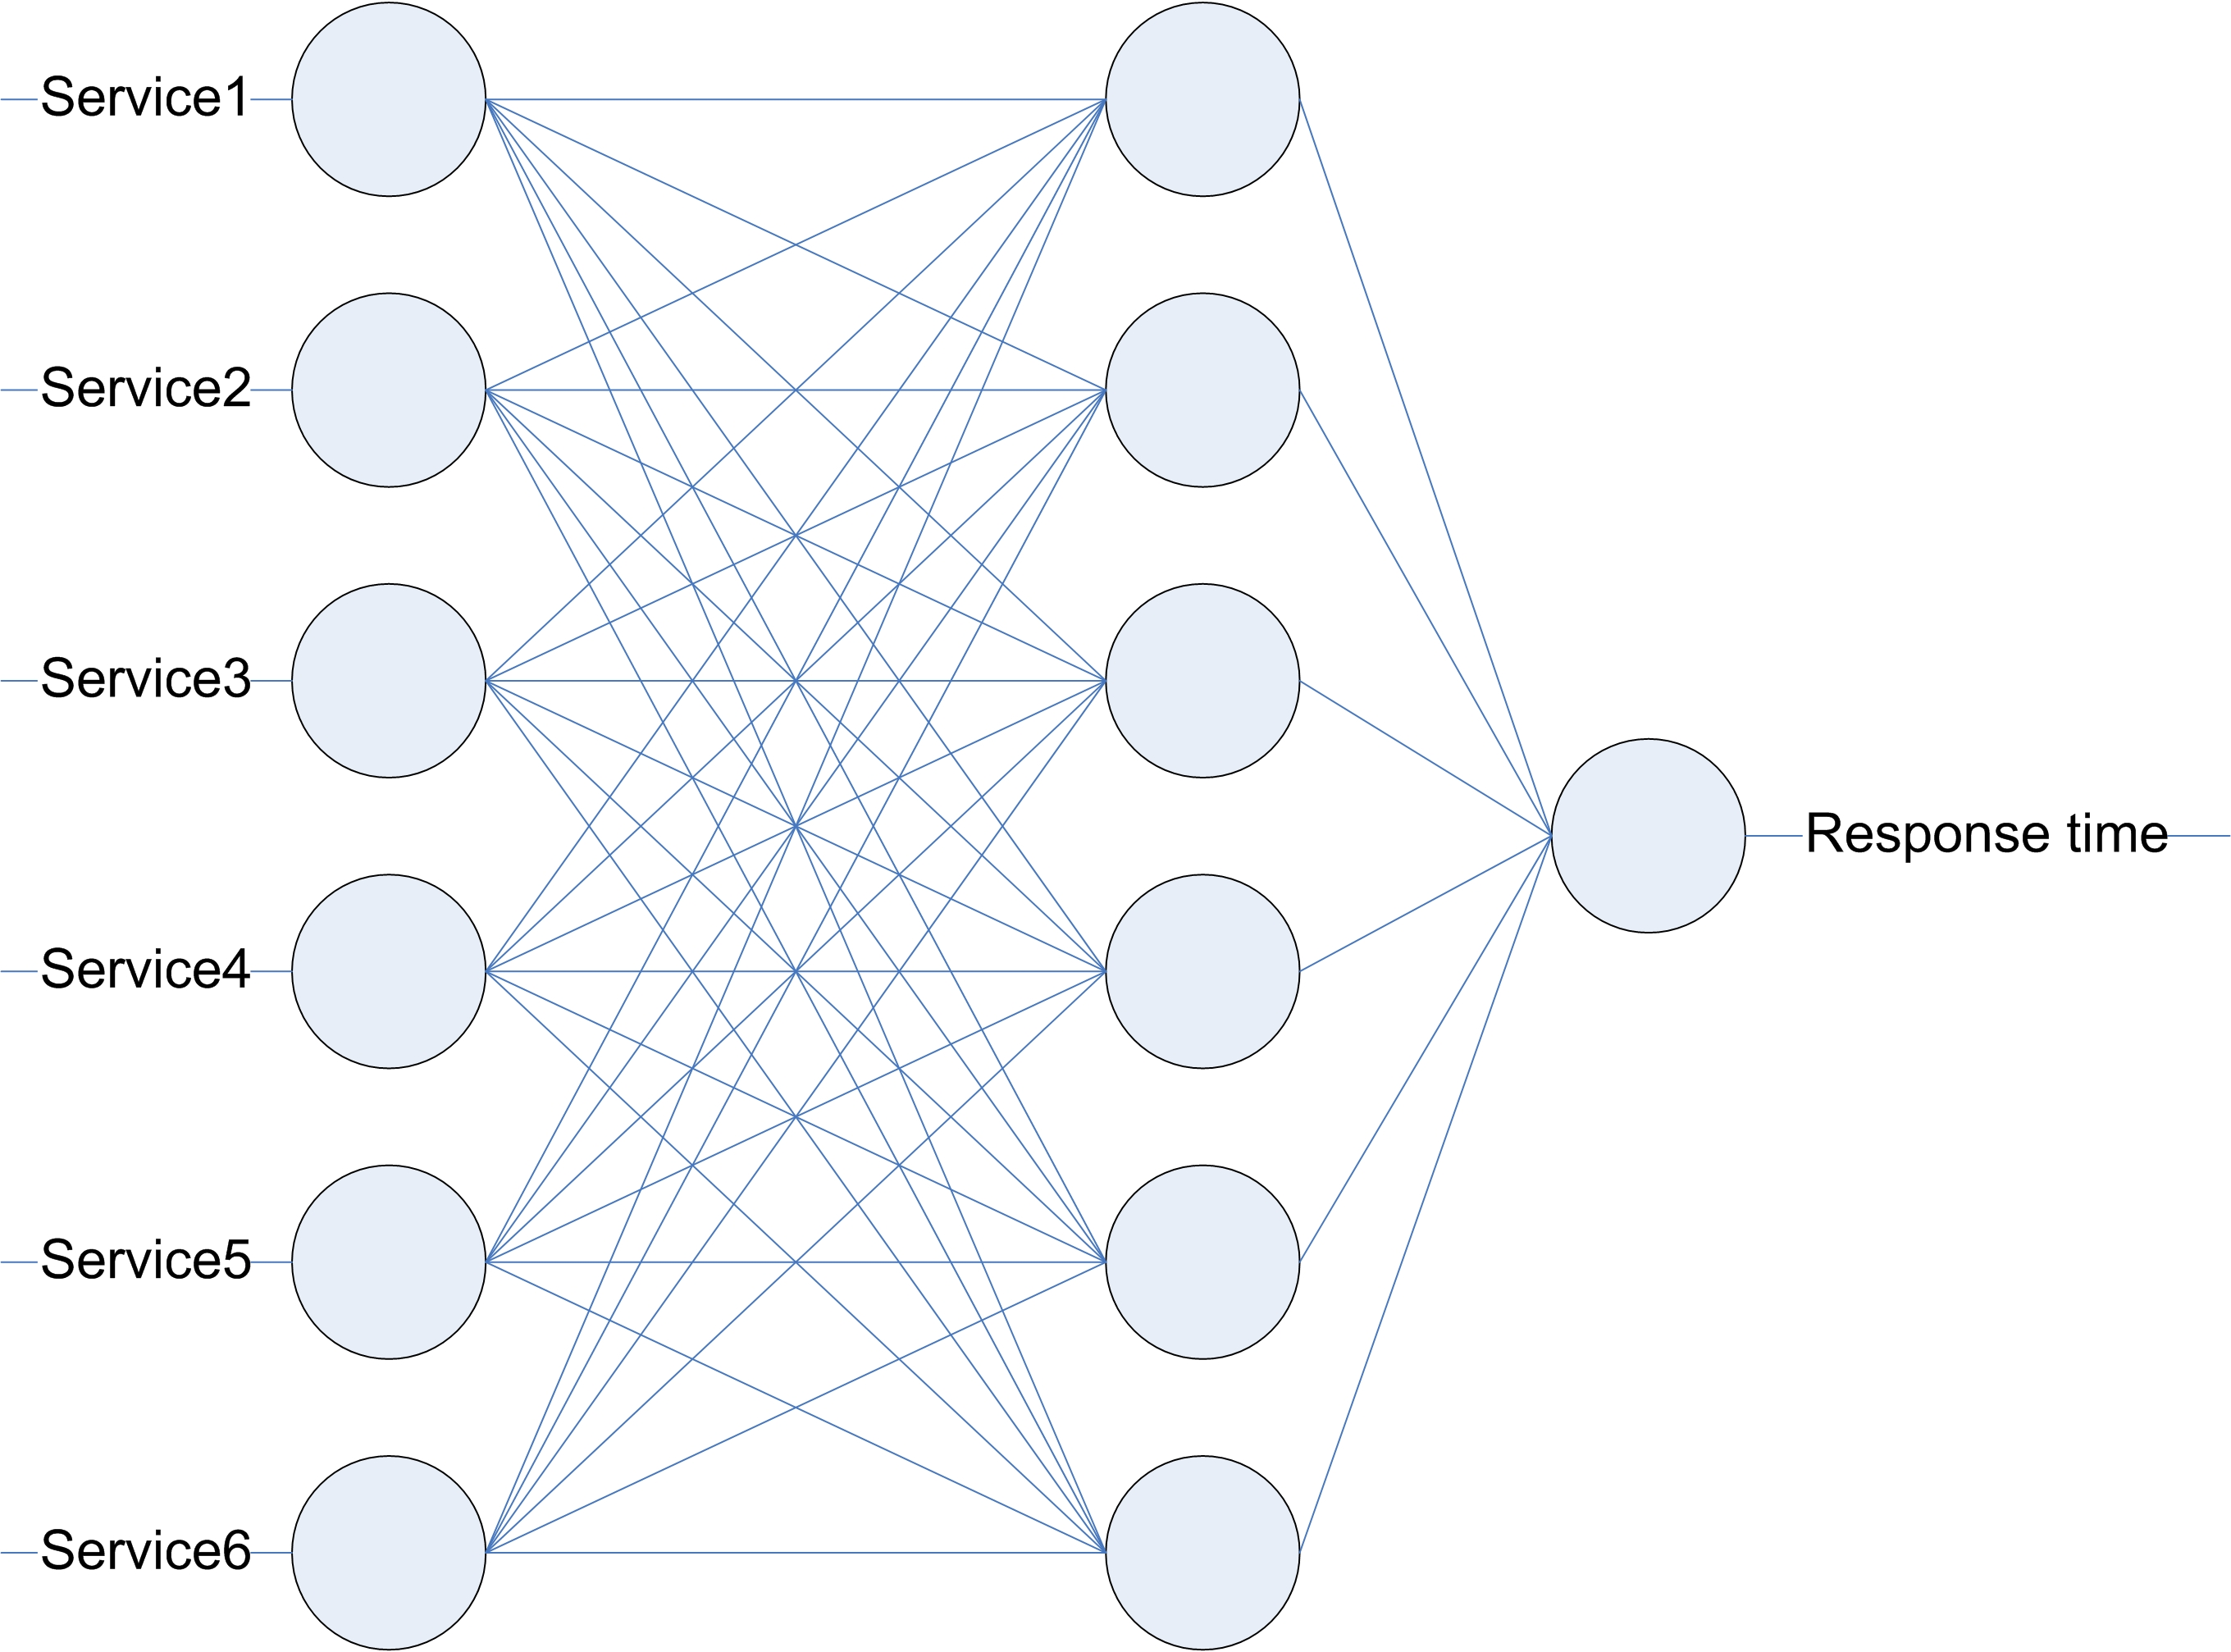
\includegraphics[width=0.65\linewidth]{neuralnetadapt}
	\caption{Neural Network Model}
	\label{fig:neuralnet}
\end{figure}

Similarly in \cite{related:bayesiandb} the authors use a Bayesian network in order to predict the response time of a database query or workload using a model which is built online and can be modified at run time. In order to achieve these goals, the authors use a Gaussian based response time model to encode the Bayesian probabilities. The Gaussian model is first trained offline and is capable of adapting itself once running online. Using a number of Gaussian models (linear and non-linear) the authors perform experiments on a database test bed and show the performance and robustness of the various models. One thing to note from the results is that all models have problems predicting queries that have not been seen before. Similarly, the models have problems making predictions when the online system is configured differently from the training system. 

\subsubsection{Layered Queueing Models}

A different approach taken to develop autonomic systems is to use Layered Queueing Models (LQM) to represent the behaviour of the system, and then to solve the LQM to predict the future state of the system. Autonomic Queueing Models base themselves on Queuing Network Model (QNM) theory, which sees an IT system as a network of queues such as CPU queues, I/O queues, network queues, etc. Requests to the system are split into a number of classes, where each class of requests exhibits the same behaviour with respect to the queues. The response time and throughput of the system can then be calculated based on the time it takes for the requests to go through the queues. A very important note about QNMs is that the structure of the queues can not be changed at run time and represents a static view of how the system must behave. As such any online adaptation in a QNM can only change the various parameters for the queues, but not the underlying structure of the queues and connections between queues. Figure \ref{fig:queueingmodel} shows a Layered Queueing Network with 3 nodes (each node has its own queue) in two layers. Arrivals into the system come into nodes 1 and 2, and from there requests move to node 3 from which the output is dispatched. Such a model can be used for two application servers with one database for example.

\begin{figure}
	\centering
		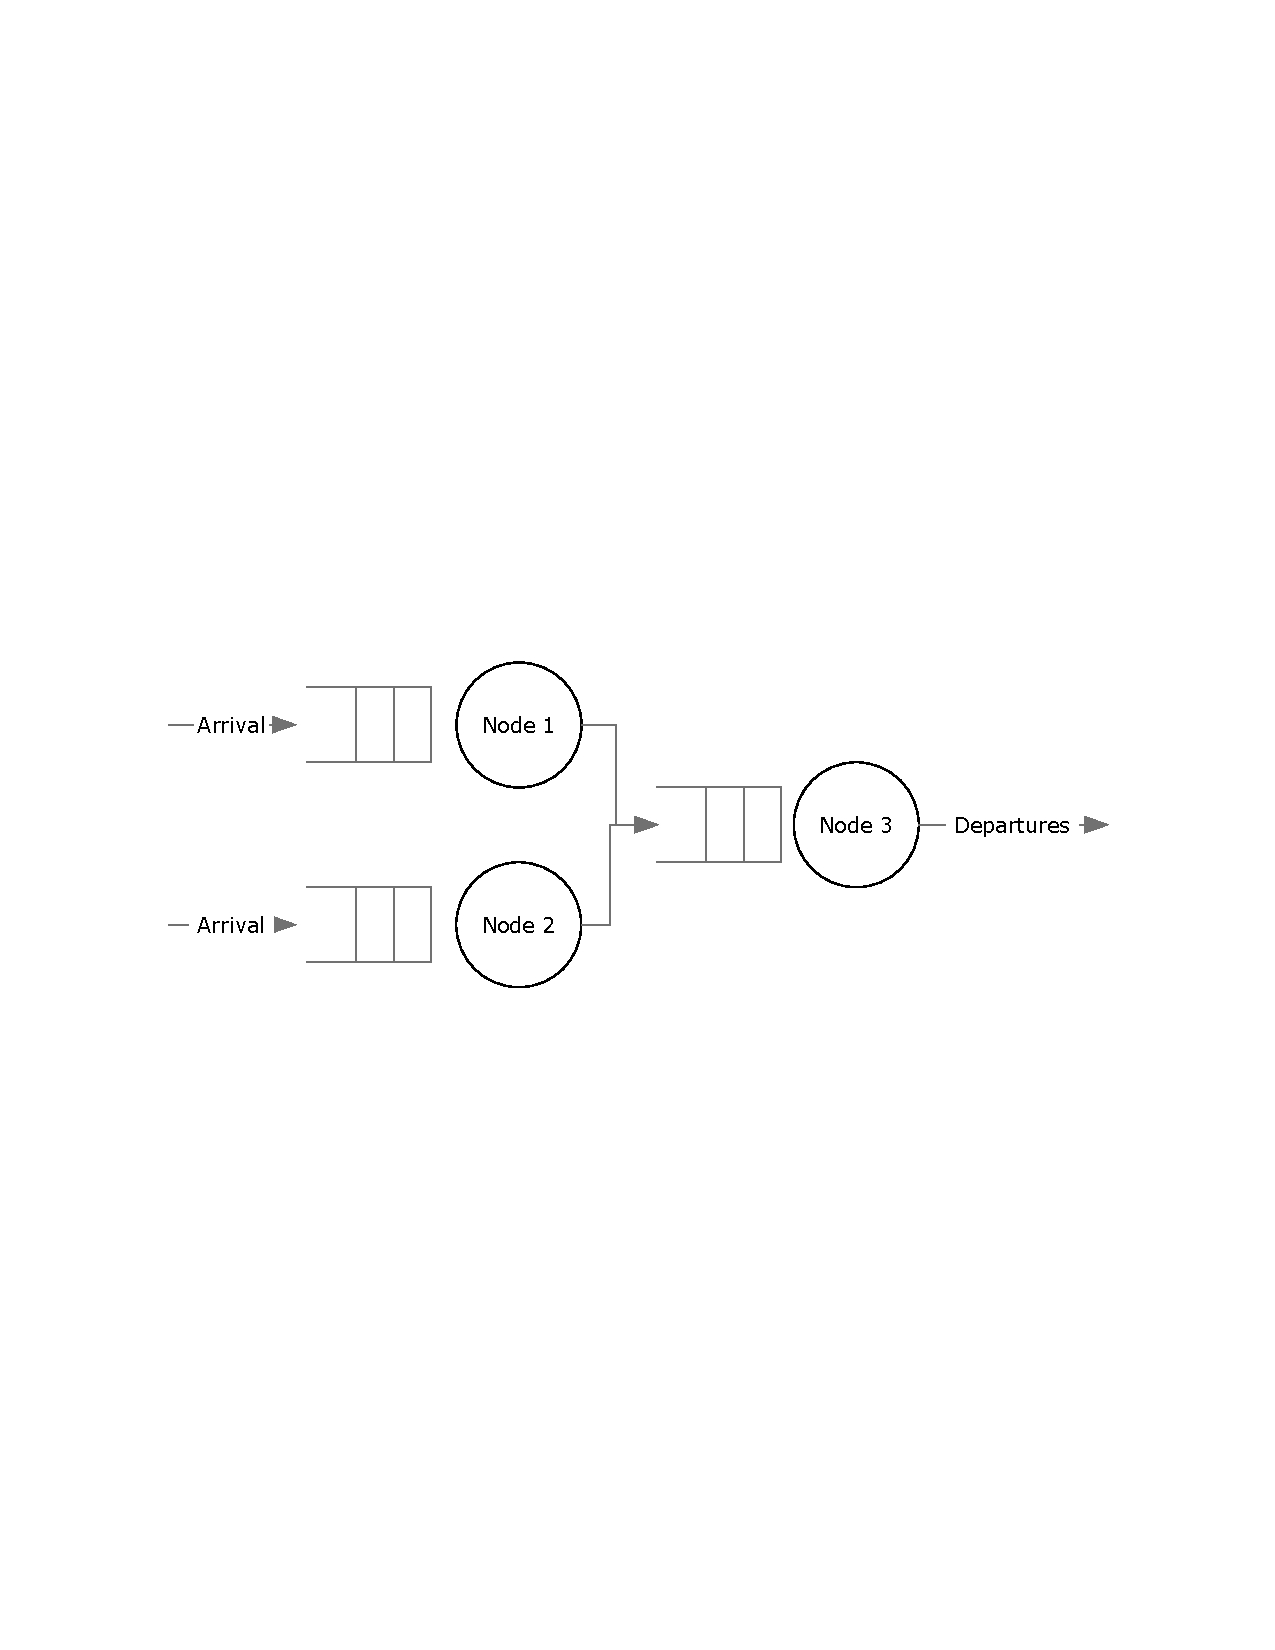
\includegraphics[width=1.0\linewidth]{ThesisRelatedQueueingModel}
	\caption{Layered Queueing Network Model}
	\label{fig:queueingmodel}
\end{figure}

Such an approach is taken in \cite{related:model:lqm} and \cite{related:model:lqm2} where the authors develop queueing models for multi-tiered transactional applications (i.e. a web server facing the client and sending requests for processing to an application server which uses a database to store and retrieve persistent data). In \cite{related:model:lqm} The LQM developed has a number of roles. First of all, the model is used to predict the future response time for each of the request classes by first predicting the future number of clients arriving in the system. If any of the predicted responses is outside the desired SLA, use the model to compute the number of servers which would alleviate the bottleneck since any high response is caused by bottlenecks at one or more of the queues. The new number of servers is computed using a hill-climbing algorithm. Finally, provision the new servers that alleviates the bottleneck problem. One thing to note, is that ``the forecasting step is in the order of minutes'', however there is no mention of what a good time period for forecasting would be or how various forecasting periods impact the forecasting accuracy. The problem in \cite{related:model:lqm2} is similar in that an LQM is build for a multi-tiered system. However, the authors develop a heuristic to try and maximize the profit obtained by the difference between revenues from SLAs and the cost of keeping servers on. This is done in part by load balancing when possible multiple similar requests to the same machines and by deciding which servers to allocate to which application tier. The authors approach is used to show results that suggest better performance than when using a proportional assignment schema. One issues that exists with this approach is that the algorithm takes a long time to find the maximum, and as such can only be run periodically and can not be used to continuously improve the system. At the same time, the authors choose a value of 60\% utilization as good utilization for the servers, but autonomic systems should attempt to obtain higher utilization in favor of using less machines, since it is preferable from an economical point of view to use one machine at 100\% than to use two machines running at 50\% each.

While the high-level modeling approach for the QNM  is very similar to the Bayesian models described previously, the differences appear in how the model is built and used. The Bayesian models output is based on the previously known probability of an observed distribution (past information on behaviour leads to the prediction of future behaviour), while the QNM's output is based only on the current size of the queues (present state of queues predicts future behaviour). The similarity between the models appears again regarding the functions that they perform. Both models are used in order to predict the future state of the system's output variables based on the current model state and a new input value, and both models can update their parametric model based on observed input and output values.

\subsubsection{Markov Chains}

A third approach, which appeared more recently in literature is that of using Markov chains, either discrete or continuous, in order to model the behaviour of the managed IT system. Figure \ref{fig:markovmodel} shows an example of a Markov Decision Process with 3 states and 2 actions. Each of the states can lead to any of the two actions, and from each action a certain probability leads to a different state. Some of the transitions have either positive or negative rewards, seen as the italic values next to some transitions.

\begin{figure}
	\centering
		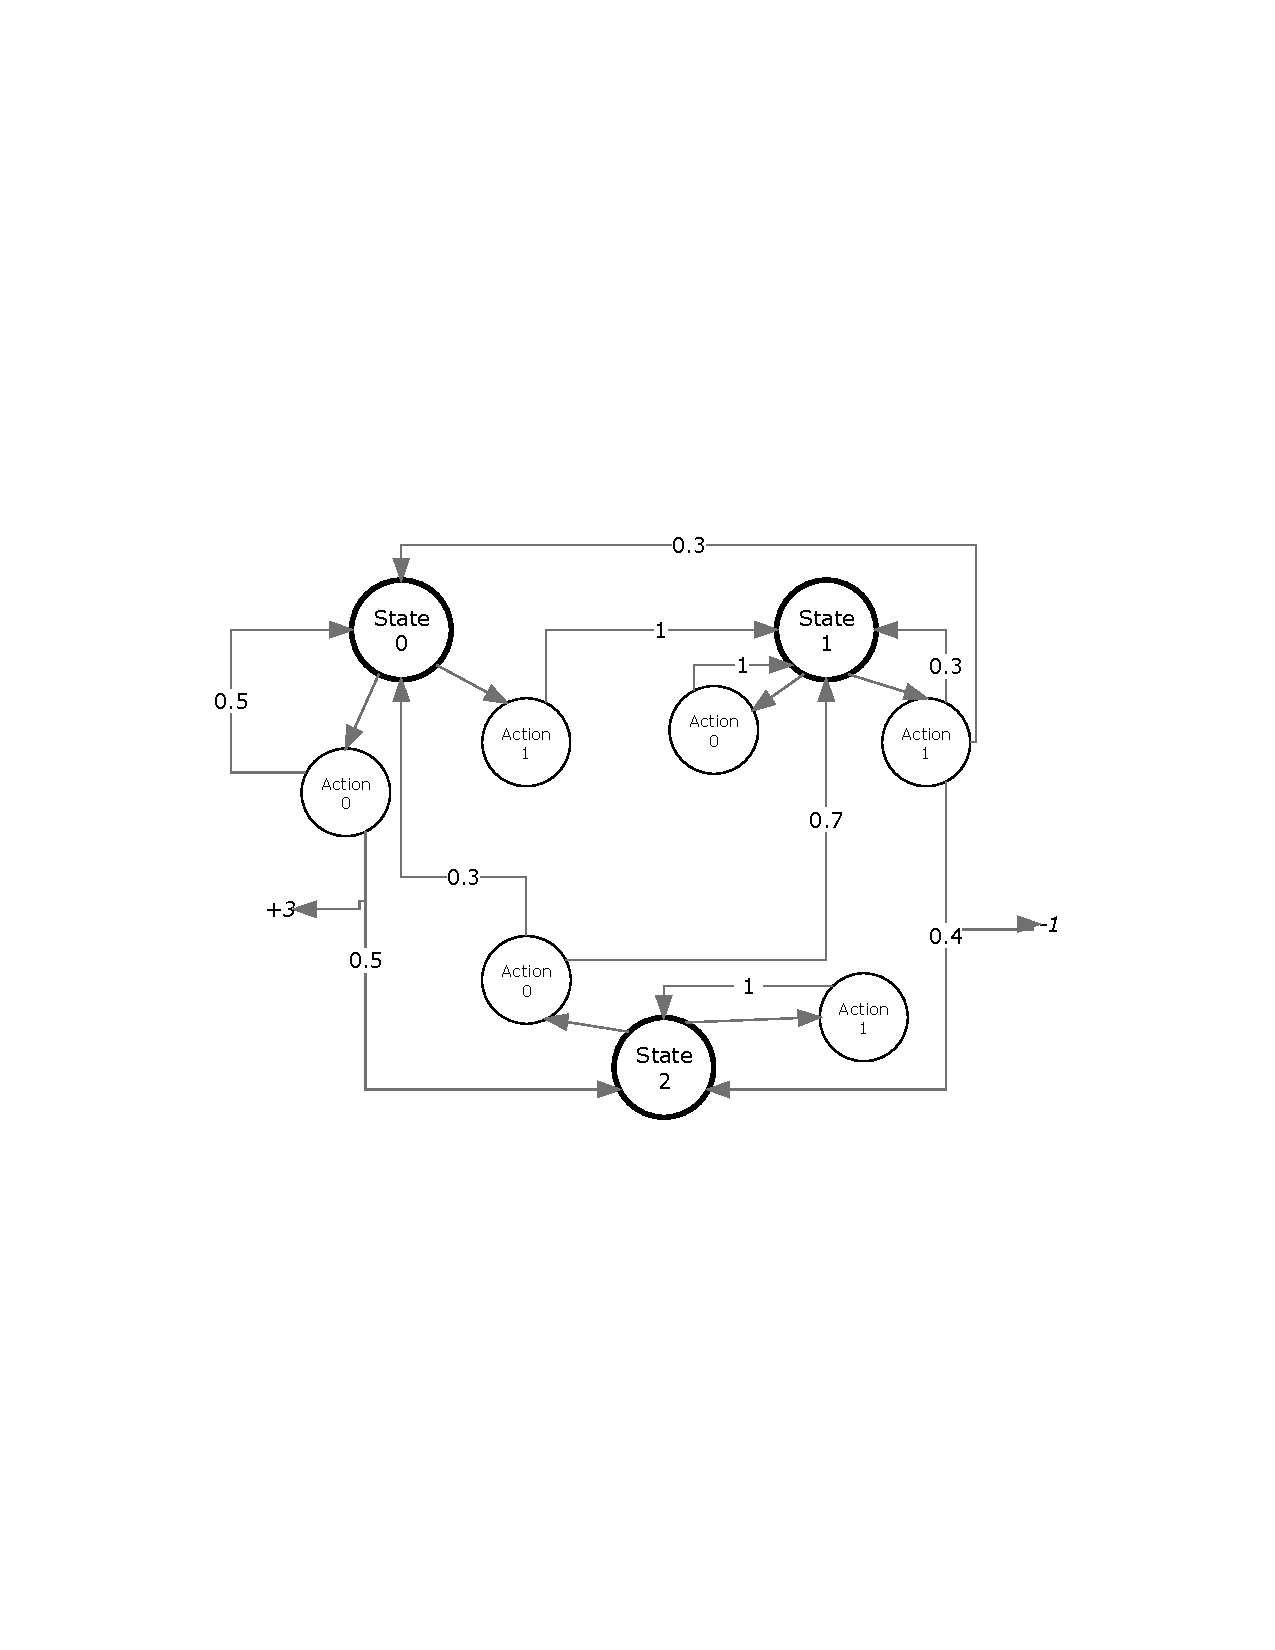
\includegraphics[width=1.0\linewidth]{ThesisRelatedMarkovModel}
	\caption{Markov Decision Process Model}
	\label{fig:markovmodel}
\end{figure}

In \cite{related:markov1} the authors introduce a framework for autonomic systems which uses Markov chains in order to model the system and by quantitative analysis of the Markov chain make decisions on how to adjust at run time the parameters of the IT system. In order to develop the system, the authors employ a probabilistic model checker/quantitative analyzer which uses a cost/rewards model to improve the parameters of the system. The autonomic system is applied to two autonomic problems. 

The first problem is that of dynamically managing the power of a hard drive by switching the state of the drive to sleep when it is idle. In experiments with the autonomic system, the management obtained using Markov chains performs better in terms of utility when compared to a simple timestamp method and N method. Also to note, the execution time of the autonomic system is sub-second but the CPU overhead is in the 1.5\% to 2.5\% range which is high for a problem like disk management. The second application of the autonomic system is for the adaptive management of a group of servers in which servers can be assigned to one of multiple clusters with clusters having different levels of SLA. The desired goal is to assign servers in such a way as to always reach the target availability of the most important cluster and trickle down in terms of cluster importance. For this purpose, a Markov chain is created for the cluster as well as a utility function which is to be maximized. A simulation is run with the described system and while the autonomic management ensures that each of the clusters has sufficient servers, the system does not deprovision unused servers. As such, the clusters have more servers than required. At the same time, based on the given results the system over-provisions the highest priority cluster by a large margin. In terms of execution, the authors mention that the system takes 30 seconds to compute the new state, which is an acceptable time to take, since provisioning servers takes an order of magnitude larger time to execute. A further issue is that it is unclear from the paper, if the system is reactive (changes the system once the SLA is breached) or proactive (predicts an SLA breach and changes the system before the SLA breach happens).

Similarly, in \cite{related:markov2} the authors use a Markovian decision process policy with reinforcement learning in order to perform resource allocation in a cloud environment. Markovian decision processes are an extension of Markov chains which allow for the existence of multiple actions for a state, thus including choice while going from one state to another, and of rewards, thus including a way to motivate the selection of a certain path. The goal of the system, is to manage a cloud datacenter, such that VMs are allocated in such a way as to maintain a required SLA for each of the applications running in the cloud while at the same time optimizing the number of VMs for each application. This problem is represented by the authors in the form of a Markovian decision process which takes into consideration the workload, the number of VMs allocated and the response time. Based on these values and the state of the decision process the system decides how many VMs to add or remove. One issue with a simple decision process is that the probability distribution functions are computed offline, and the system simply uses the predetermined functions to compute an optimal policy. The authors alleviate this problem by using a reinforcement learning approach to update the probability function by using rewards for good decisions. The authors apply the system on a simulation of a cloud with one application. The Markovian decision process system is capable to reach a policy which ensures that the SLA is maintained quite quickly. However, it is unclear if this allocation is optimal, since in the graphs the response time is 20 - 40\% lower than the required SLA, which could simply be due to over-provisioning of VMs. One interesting note of the authors is that long running systems will exhibit major changes in behaviour when the model has to be changed entirely since a reinforced learning system will not be able to react promptly due to the ``old'' knowledge in the system. At the same time, the authors note that the information used as input for the system is insufficient for appropriate decision making in the real world, as more data from the environment will be needed.

\subsubsection{Economic Models}

A similar approach to a punishment/reward system in order to make decisions is that of using economic models in policy making. Economic models consist of two actors: suppliers and consumers which use a trading mechanism to exchange resources. The trading mechanism is usually based on some form of ``currency'' which consumers use in order to obtain resources from suppliers. In \cite{related:econmodel} the authors apply an economic model in order to translate between business policy and low-level requirements for the automation of a database system. The control goal of the system is to tune the buffer pool of the database as well as the CPU usage when faced with multiple workloads. The workloads act as consumers and each workload has its own buffer pool and its own set of database agents, but the system does not have enough resources for all the workloads to execute quickly. Each workload has an estimated wealth based on the relative importance of the workload and the estimated work required for the workload, which is calculated based on the database's query optimizer prediction of I/O operations for the query. Using this wealth consumers (workloads) bid on resources dependent on the marginal utility provided by the given resources until either no more resources are available, the consumer uses all its wealth or the consumer has sufficient resources. A resource broker is used to enable the bidding process. The resource broker divides all the resources into blocks of resources which are up for bidding. For each of the resource blocks, the resource broker receives sealed bids from the consumers and chooses the highest bid. The bidding process repeats until no more resources are available, no more resources are desired by consumers or consumers do not have any wealth remaining. The above system is validated by running tests on an experimental environment. The economic model is first used to determine the resource allocation offline and the database is configured based on the results of the economic model. It should be noted that the system is not used to update the database's configuration online based on changes in workloads. The authors observe that the developed system is capable of obtaining effective allocations which result in similar number of reads to a system configured manually, which respect the desired importance of workloads and which result in the expected relative performance with respect to the relative importance values. One problem which the authors observe with the system is the fact that a real system would not know ahead of time the possible workloads (if such knowledge was available ahead of time manual configuration would be sufficient) and as such the utility functions would be hard to determine at run time. To create a really autonomic system a feedback loop would be required to obtain statistics from the running workloads and update the utility functions.

Another solution for autonomic systems is based on cost functions and optimization of such functions. In \cite{related:model:lqm2} which also uses a Layered Queueing Model and was described previously such a method is described. The authors assume that in a data center there are various costs: energy, hardware, and software utilization, as well as revenues obtained by providing the service and penalties due to breaches of SLA. The plan function is then based on the observation that ``revenues increase almost linearly with the system load and start decreasing after a maximum that is obtained when the service center utilization is about 0.5 to 0.6''. Because of this, the plan function attempts to optimize the cost function but since the optimization problem is NP-hard, the solution proposed is a heuristic search which results in a local optimum, but not necessary the global optimum. One important aspect of this paper is that it shows how multiple methods can be combined to create autonomic systems. In this case an economic based policy on top of a queueing model of the datacenter.

\subsubsection{Control Theoretic Models}

Due to the fact that autonomic system architectures are based on the MAPE-loop an approach to develop such systems which maps extremely well on the MAPE loop is that of using control theory methods and algorithms. One very important aspect of developing a system based on control theory (which also applies to some of the other methods) is that of creating a model for the system. Figure \ref{fig:blackbox} shows an example of a black box model for an application server. The arrival of clients acts as a perturbation on the system, which will change the internal state of the system which is hidden by the black box and in response to the state change the outputs of the system - CPU utilization and response time will be modified.

\begin{figure}
	\centering
		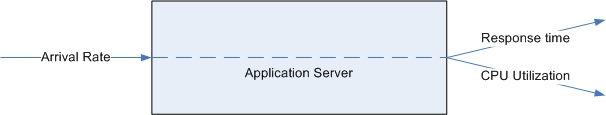
\includegraphics[width=1.0\linewidth]{BlackBox}
	\caption{Server Black Box Model}
	\label{fig:blackbox}
\end{figure}

The authors of \cite{related:control} explore how control theory can be applied to systems research in order to develop a management system for cloud computing environments. The authors note that such an environment, in which applications are consolidated across virtual machines and share dynamic resources based on the changing workload for the applications, pose a number of challenges to system administrators in the form of: ``complex SLAs, time-varying workload demands, distributed resource allocation and resource dependencies''. These challenges are addressed by using control theory in order to model, analyze and design a feedback loop for a resource management system. The autonomic system developed is applied to the problem of resource allocation in a shared virtualized infrastructure. The system does not provision new servers for the various applications, it just changes the resource allocations for the various virtual machines dynamically. The goals of the system are to guarantee application performance by reaching all the desired SLAs for the applications if possible (high demand periods could cause all resources to be used and low priority applications to miss their SLAs) and to provide high resource utilization and performance differentiation during contention periods (high priority applications maintain their SLAs over low priority applications). The authors identify six strengths of the control theoretic approach for autonomic systems, which are:

\begin{enumerate}
	\item Control theoretic systems offer a quantitative input-output model where a black-box model can be developed by performing offline experiments in order to determine the relation between the given control input, the perturbations in the system and the observed outputs which are the values to be controlled. Use of a proper input-output model in relation with a feedback controller offer the advantages of ensuring that the system converges towards equilibrium, that the system is stable and converges in appropriate time and that the controller can adapt to different regions of the input-output relation (for example if the input-output relation is bimodal).
	\item Control theory offers the ability to study system dynamics, which refer to the transient effects of past states on the current system state. Such input-output models can also be built by using system identification experiments to determine the degree of correlation between current output and past output values.
	\item Furthermore, using control theory system designers can develop multiple-input and multiple-output (MIMO) control models in order to capture the relations between the various inputs and outputs of the system. The relations in such systems are hard to quantify even when they are known.
	\item Control theory provides a number of well researched and well investigated algorithms for control based on models discovered via system identification for both single-input, single-output (SISO) and MIMO systems.
	\item Control theory also offers methods to determine the stability of the closed-loop model and control system. At the same time, control theory deals with the tradeoff between stability and responsiveness of the control system which is the tradeoff between how fast the system reaches a change decision and how stable the control system's decision is. A system which reaches decisions too fast will oscillate and be unstable as any small change in perturbations will result in a control decision. On the other hand a very stable system will make changes very slowly and miss important changes in perturbations.
	\item By using adaptive control theory, system administrators can develop controllers for systems with varying behaviour over time. This can be done by estimating the parameters of the model online and attempting to keep the parameters in line with the actual state of the system.
\end{enumerate}

For each of the six strengths the authors offer examples of how they applied control theory to various autonomic problems. The authors however, also note some limitations of control theory which must be taken into account while developing autonomic systems. First of all, computer systems exhibit non-linear behaviour which makes modelling more difficult. Second of all, the development of black-box control models requires very controlled experiments to be run. Such experiments can not be usually run based on data from production systems since such data rarely contains the required perturbations or constraints to determine the relations between input and output. Third of all, classical control theory deals with continuous inputs. While discrete values can be quantized, this can lead to instability or inefficiency. Finally, classical control theory usually deals with tracking problems - the control system maintains a variable at a certain value. For autonomic systems, the goal is generally to maximize or minimize some values (maximize resource usage while minimizing response time for example). Any person who creates autonomic systems by using control theory must take these limitations in consideration and deal with them.

Similarly, in \cite{related:control2} the authors compare various approaches to creating decision makers for autonomic systems. They look at heuristic approaches, standard and advanced control-based approaches as well as model-based and model-free machine learning approaches. In order to compare the five methods the researchers look at a standard autonomic computing problem, namely the problem of resource allocation to some running application in an operating system. The application which is assigned resources has a way to signal ``heartbeats'' at important places in code as well as to describe desired performance goals. The authors conclusion is that an adaptive control approach like a Kalman Filter produces good results for a range of applications, and this matches the observations of \cite{related:control}. The authors note that for a given system with a narrow range of behaviours testing multiple approaches is the best approach, for a system with a broad range of behaviours or even unknown behaviour ahead of time (a self-optimizing application server with unknown applications running on top) adaptive control is the best approach.

The issue of applying control theory methods for managing the CPU shares received by multiple resource containers running on the same machine is addressed in \cite{related:control3}. Resource containers are a way to provide performance isolation for applications running on the same hardware and they can be either an operating system feature or an entire technology like virtualization. Usually the resource container resource allocation is done offline before deployment and does not change during the lifetime of the applications. The authors present an approach to change the resource allocations dynamically by using a feedback control loop based on control theory principles. The specific application under control in this case is an Apache Web server running inside HP-UX PRM as a resource allocation system. The model of the system is created by applying system identification on observable metrics for a black-box model. The reason to use a black-box model given by the authors is that the complexity of a web server makes it hard to obtain a control model from first principles. The model for the system is a SISO model which correlates the CPU usage of the resource container to the Mean Response Time (MRT) of the web server. The system identification is done using a single workload meant to stress the CPU of the container. Using the model obtained by system identification, the authors apply a simple Proportional-Integral (PI) controller and show that such a system is stable, has a rise time of 3 sample periods and settling time of 6 sample periods. The rise time refers to the time it takes for the controller to respond to a change in perturbations, while the settling time refers to how fast the controller reaches stability after a perturbation.

The problem with the PI controller is that it is ``trained'' through system identification on one workload and would not respond very well to a different workload. In order to deal with unknown workloads the controller must be developed using adaptive control. This observation matches that of \cite{related:control} and \cite{related:control2} which note that adaptive control is best for systems with unknown behaviour ahead of time or for those with changing behaviour. The adaptive control is applied to the system by adding a parameter estimator for the model discovered using system identification. The two parameters are estimated using the recursive least-square (RLS) method and are updated at each interval. The parameters are then fed into a pole placement module which chooses the desired parameters of the PI controller in order to have the poles of the transfer function at the desired location. The two control systems (adaptive and simple PI) are evaluated on a test-bed. The simple controller is capable of maintaining the response time within 15\% of the target value when being faced with a workload similar to the one used for system identification. The adaptive controller is capable of maintaining the response time within 20\% of the target value even with changes in the workload. However, the tradeoff is that the convergence towards the desired response time is slower using the adaptive controller and that this controller also oscillates more. The simple controller is not tested on the varied workload since its results would be bad.

\cite{related:control4} deals with a similar issue, that of developing a feedback control system for managing the service delay (response time) for web servers based on relative or absolute delay guarantees. Absolute delay guarantees require that each class of services is served within the desired time when the server is not overloaded. When the server is overloaded admission control is applied based on some form of priority order over the services. In relative delay a fixed ratio between the delays of the various classes is maintained. The problem with ensuring such guarantees is that the workload is unknown ahead of time, and as such developing a robust control system for service delay guarantees is complicated. Two types of controllers are used in the proposed system - one for relative and one for absolute service delay. The absolute delay controller uses a PI controller similar to the work in \cite{related:control3} and the control parameters are determined using system identification. The relative delay controller computes the relative delay between two adjacent classes. Thus the system contains n-1 controllers for n classes of services. Each of the controllers uses a PI controller with extra logic on top to calculate the ratio of the two service classes under control. Similar to all the other control theoretic papers, the authors note that such a system would face problems if the workload during deployment is vastly different from the workload on which system identification was done. In order to alleviate this issue one can use adaptive control. The system is applied to a testbed of Apache Web Servers for both absolute and relative delays with two and three classes. The experimental results show that the control method is capable to reach the desired guarantees when run in a closed-loop, while the open-loop solution violates the desired delays when the workload changes.

Similar work is performed in \cite{related:control5} where the issue of managing the database connection pool in a web server is approached from a control theoretic point of view. The goal of the work is similar to that of \cite{related:control4} in that the system's final goal is to improve the response time of a server under heavy load. Unlike \cite{related:control4} this is achieved by setting priority for the idle connections in the database connection pool, however similar to \cite{related:control4} this is done by using the dual approach of proportional delay differentiation and absolute delay differentiation. Like \cite{related:control4} the authors use system identification to determine the PI controller's parameters by applying the RLS method. The system is tested on a server running Tomcat and the system is capable to maintain the desired response time in the face of varying workloads.

Based on this work a number of observations about control theory for autonomic systems can be observed. First of all, all research in autonomic systems control theory has focused on developing black box models due to the difficulty of applying first principles to IT systems. Second of all, most researchers focus on using simple controllers like the PI controller for autonomic systems and use experiments and system identification in order to find the parameters of the controller. In order to deal with varying perturbations, researchers apply adaptive control on top of the simple PI controller.

\subsection{Self-organizing Systems}

Self-organizing systems deal with complexity in management systems by allowing the management of the system to appear from the interaction between the components of the system. Such systems have no global controller and components do not have access to information outside their own local information. Components can however exchange messages with each other to inform other components about the sending component's state. Through this, ``emergent'' behaviour appears in systems, behaviour which is not imposed from outside the system. Like autonomic systems, self-organizing systems are inspired by behaviour observed in nature like ``synchronous flashing that sometimes develops among aggregations of thousands of fireflies in southeast Asia'' or the stripped and mottled pattern which appears in zebras and fishes. Experiments and theoretical work suggests that such apparent complex patterns appear from a small number of very simple rules and research into them can be found in \cite{related:selforganization-honeybee}, \cite{related:selforganization-autoscaling}, \cite{related:selforganization-autoscaling2}, \cite{related:selforganization-plant}, \cite{related:selforganization-healing1}, \cite{related:selforganization-healing2}, \cite{related:selforganization-energymanagement}.

The problem of the stripped pattern was examined in computing by Alan Turing who first suggested in 1952 the general schema for this mechanism of self-organized pattern formation. The self-organizing system has a number of sites which act as activators. The activators produce two pheromones: a short range activator which enhances the activator production and a short range antagonist which ensures that the self-enhancement is localized. By performing simulations using a model of such a system both stripped and mottled patterns can be obtained. This shows that complex behaviour can emerge from very simple rules through the collaboration of components.

Self-organizing systems were also employed by Ashby to create his homeostat \cite{ashby:homeostat} which is capable of adapting itself to any perturbation in the system and reach back a stable state. The initial system built by Ashby was an adaptive ultra-stable system with the goal of showing Ashby's law of requisite variety, which states that a control system needs as many internal states as those of the system being controlled. The system automatically adapted its internal configuration to stabilize any disturbance introduced in the system. Figure \ref{fig:homeostat} shows the output of a homeostat. As any of the four pens is perturbed, the system self-organizes until all four pens are back to a stable state.

\begin{figure}
	\centering
		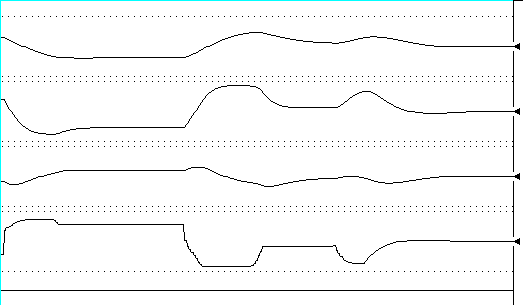
\includegraphics[width=1.0\linewidth]{homeostat}
	\caption{Homeostat}
	\label{fig:homeostat}
\end{figure}

In \cite{selforg:survey}, the authors look at a number of self-organizing algorithms and compare them in the context of the problem of load balancing requests in a cloud environment. Some of the algorithms examined include Particle Swarm Optimization, Artificial Bee Colony, Genetic Algorithms and Ant Colony Optimization. Furthermore, the authors examine in detail the Ant Lion Optimizer algorithm for load balancing due to it's better performance and better ability to search the entire solution space instead of falling into a local optima. The authors observe that the self-organizing algorithms perform better than traditional algorithms in terms of quality of service provided and minimize the response time, at a tradeoff of more network and processing overhead.

\subsubsection{Genetic Algorithms (GA)}

One of the oldest approaches for self-organizing systems is based on mutating solutions and maintaining only the fittest solutions to continue mutating in the future. The optimization usually starts with a random solution which is encoded in some form of digital representation - usually a binary string. There also exists some form of fitness function which decides how good a solution is. Solutions are chosen in pairs and they exchange part of the solution to form two children. Mutations can also be introduced by randomly changing part of a child. After the population of children is obtained, the children are measured using the fitness function and unfit children are removed from the population. The surviving children become the new parents and the loop is repeated either for a given number of iterations or until a certain fitness value is passed. The final solution is the one with the best fitness of the entire population. The pseudocode in \ref{algo:ga} shows the behaviour of GA algorithms.

\begin{algorithm}
\begin{algorithmic}
\State Random generation of initial parents
\While{end criteria not met}
	\State Select parent pairs and cross over chromosomes
	\State Randomly mutate children
	\State Compute children fitness
	\If{child is fit}
		\State keep child in population
	\Else
		\State remove child
	\EndIf
	\State replace parents with children population
\EndWhile
\State return best fit child
\end{algorithmic}
\caption{Genetic Algorithm Pseudocode}\label{algo:ga}
\end{algorithm}

In the case of the problem presented in this thesis - that of optimizing the size of a cloud of servers dynamically at runtime - a GA could encode the servers to be used as a binary array of 0 or 1, and then find the best solution in terms of future performance of the system by predicting which servers should be up (a 1 in the binary array) or stopped (a 0 in the binary array). The GA can not be used in order to determine when the system is about to breach its SLAs, and can only be used in order to obtain a new optimal state. At the same time, GAs are known to be slow in order to obtain a good solution as the number of iterations taken to converge can be very large if a good solution is desired. As such, GAs are not a very good fit for a real time self optimization of cloud resources.

\subsubsection{Particle Swarm Optimization (PSO)}

Particle swarm optimization uses as inspiration the behaviour of flocks of birds or swarms of fish looking for food. Each possible solution represents a particle in the search space with a position, and the particles move based on their own speed and the best known position. At the same time, there exists an optimization function $f$ which takes as value the position of a particle and returns a value representing how good that solution is. As such, each particle is initialized with a random position and speed. Each of the position computes it's $f$ function and save it as the position's best solution. The best of the $f$ values is stored as the swarms best solution. At each step of the iteration, each of the particles computes a new speed and a new position based on the previous position and speed, such that each particle's movement is guided by it's own best solution and the swarms best solution. Once an exit criteria is reached - either number of iterations or the desired function is sufficiently improved, the algorithm exits and the best swarm position is used as the solution of the optimization problem. The pseudocode in \ref{algo:pso} shows the behaviour of PSO algorithms. $f(swarm)$ is defined as the best solution for the swarm.

\begin{algorithm}
\begin{algorithmic}
\State Random uniform generation of initial positions and velocities in search space
\ForAll{Particles} 
	\State Compute particle's position and save as best position
	\If{$f(particle) > f(swarm)$} 
		\State update $best(swarm)$ = particle
	\EndIf
\EndFor
\While{end criteria not met}
	\ForAll{Particles} 
		\State Compute particle's new speed
		\State Compute particle's new position
		\If{ $f(particle_{new}) > f(particle_{best})$ } 
			\State update $particle_{best}$ = $particle_{new}$ 
		\EndIf
		\If{ $f(particle_{new}) > f(swarm)$ } 
			\State update $best(swarm)$ = $particle_{new}$
		\EndIf
	\EndFor
\EndWhile
\State return $best(swarm)$
\end{algorithmic}
\caption{Particle Swarm Optimization}\label{algo:pso}
\end{algorithm}

For example, a PSO is used in \cite{selforg:pso} in order to obtain the initial placement of tasks in a cloud. The system described in the paper does not perform any real-time optimization and only takes care of the initial problem of placing N SaaS tasks on M cloud instances, where $M < N$. The system uses a position vector to describe which task is assigned to which server and then uses the PSO algorithm to find the best placement.

Similarly to the GA algorithm, the PSO algorithm can not be used in order to detect when a system breaches it's SLA and can only be used once some other system detects a possible SLA breach. PSOs can also fall easily into local optima depending on how well the parameters of the problem are set at the beginning. If the parameters cause too small speed/position changes than the system can fall into local optima easily. If the parameters cause large changes then the optimization problem can fluctuate.

\subsubsection{Artificial Bee Colony (ABC)}

The artificial bee colony algorithm \cite{selforg:abc} is inspired by the process used by a honey bee swarm in order to forage for food. Unlike in other self-organizing systems, not all the composing parts are the same in the ABC algorithm. Three types of bees are used in the algorithm: employed bees, onlooker bees and scout bees. The problem to be optimized is defined in terms of food sources, with different solutions representing different food sources. For each source of food there is one employed bee which goes to that source, forages and returns home. Onlooker bees stay at the nest and establish new food sources based on the information received from employed bees returning to the hive. Onlooker bees choose new food sources by watching the employed bees come back to the hive in the dancing area, and perform a dance based on how good the food source is. Finally, scout bees establish new food sources via random searching around the hive.

Algorithmically, this behaviour is represented by an iterative loop over three phases: employed bee phase, onlooker bee phase, scout bee phase. Initially, the food sources are initialized by having the scout bees go and find random solutions in the solution space. In the employed bee phase, employed bees generate new solutions by going to an existing solution and searching the space around it for a new solution. Once a new solution is generated, the fitness of the new solution is computed and a greedy algorithm used to choose between the new solution and the original source. Employed bees then go to the hive and share the information with onlooker bees in the dancing area. In the onlooker bee phase, onlooker bees choose their food source based on the information received from the employed bees. Once an onlooker bee chooses a source, it also determines a neighbour and computes the fitness of the new solution and chooses between the new solution and the old. In the scout phase, employed bees which can not improve on their solution after a number of iterations give up and become scout bees. Scouts search for solutions randomly.

The pseudocode in \ref{algo:abc} shows the behaviour of ABC algorithms.

\begin{algorithm}
\begin{algorithmic}
\State Initialize solutions randomly using scout bees
\While{end criteria not met}
	\State Employed bee phase
	\State Onlooker bee phase
	\State Scout bee phase
	\State Store best solution up to now
\EndWhile
\State return $best(solution)$
\end{algorithmic}
\caption{Artificial Bee Colony}\label{algo:abc}
\end{algorithm}

Like the GA and PSO algorithms, this algorithm can not be used to detect problems in the system, and can only be used to obtain an optimal solution to the problem at hand. Compared to both GA and PSO, ABC offers similar or better performance but with less control variables needing to be used - thus creating a simpler algorithm to implement.

\subsubsection{Ant Based Algorithms}

Similar to the ABC algorithm, the ant colony optimization (ACO) algorithm is inspired by the behaviour of insect hives - in this case ants. The behaviour which inspired this algorithm is the way in which ants can build an efficient path between the nest and a food source using random search and reinforced learning. In real life, ants randomly search for food around the nest. When an ant finds a food source it returns to the nest with some food while laying a pheromone trail. Other ants which meet the pheromone trail are more likely to follow the trail then continue searching randomly. If the food source is large enough eventually a large number of ants follow the same path as each ant lays down a pheromone trail causing more ants to follow it. At the same time, the pheromones dissipate over time such that once a food source is depleted and ants no longer return with food from it, the trail will disappear. 

The ACO algorithm is very similar to the behaviour of ants in real life and is best used to find optimal paths through graphs. For example, the algorithm has been used to provide reinforced learning for routers in a network for better packet forwarding \cite{selforg:aco}. In simple terms, the ACO is composed of a number of ants which are traversing the network by moving from node to node across edges. As ants move through the network they deposit pheromones on the edges based on some function. When ants decide the next node to go to, they choose based on the pheromones on the nodes going out from the current node. The selection of the next node is done pseudo-randomly such that not all ants follow the same path, however more ants will prefer edges with higher pheromone levels. 

In the case of routing in a network, the nodes are the routers and the edges are the connections between the routers. Ants are packets being sent between the routers and either they wait in a normal queue or have higher priority than normal packets. If the ants simply wait in the queues to be processed then they can measure the processing latency at the routers. As ants traverse the network they can update the routing table with information regarding how loaded is the network and also the best routes between different nodes. The pheromones in this case act as a way for more ants to go through low loaded network links such that those links are used by normal traffic.

The pseudocode in \ref{algo:aco} shows the behaviour of ACO algorithm from the perspective of an ant.

\begin{algorithm}
\begin{algorithmic}
\While{end criteria not met}
	\State Find next node based on pheromones/random
	\State Go to next node
	\State Update pheromones for the edge just traversed
\EndWhile
\State return $best(solution)$ based on pheromones
\end{algorithmic}
\caption{Ant Colony Optimization}\label{algo:aco}
\end{algorithm}

Another self-organizing algorithm is based on the behaviour of ants when relocating to a new nest in the case when the old nest was destroyed. This behaviour is similar to that of honey bees when relocating \cite{selforg:antreloc}. When their nest is destroyed, ants start looking for a new nest by doing tandem runs. In such a case, there are two types of ants - scouts and non scouts. Scouts start to search for new nests randomly and upon finding a new possible nest they determine how viable the new nest is and return home. Upon coming back home ants recruit from the non-scout ants and do tandem runs together. At the same time scout ants can be recruited by other scouts who have a better nest as their new nest. This process is repeated until a quorum of ants has chosen a new site for the nest. Ants can give up on their possible new nest if the population of the new nest starts decreasing - suggesting that ants from this new nest have been successfully recruited by a better nest. The pseudocode in \ref{algo:antreloc} shows the behaviour of the ant relocation algorithm.

\begin{algorithm}
\begin{algorithmic}
\State Round 1: Ants find new nests
\While{more than one nest}
	\State Round 2: Viable ants return home and recruit from the other ants
	\State Round 2: Not viable ants wait one turn
	\State Round 3: Tandem runs to new nest. Upon arrival at new nest ants compare previous and new nest size. Nest with decreasing pop become not viable. 
	\State Round 3: Not viable ants return home
\EndWhile
\State return $single nest$
\end{algorithmic}
\caption{Ant Colony Relocation}\label{algo:antreloc}
\end{algorithm}

The main reason to use self-organizing systems for autonomic system development is that the two have a number of characteristics in common like the ability to deal with unexpected changes in the environment. Unlike the other self-organizing systems presented, the ACO algorithm can be used to detect when the system breaches or is about to breach it's SLAs. As ants move around the system, they can take measurements and approximate the state of the entire cloud based on their knowledge of the pheromone levels across the cloud. Once a certain threshold is reached ants can trigger a request for self-optimization which is computed by a separate algorithm. Because of these reasons, this thesis will use the ACO algorithm to develop the self-organizing, self-optimizing system.

\subsection{Cloud simulation systems and benchmarks}

In order to test any proposed system and prove the performance of the system, the system must be run either on a simulation or on a live test bed. For cloud systems it is especially difficult to use a live test bed as a large number of servers or resources must be used at a significant cost. As such, a number of simulation platforms have been developed by various research groups. Furthermore, in order to be able to show that one solution is better than another a comparison must be done between different solutions.

A number of cloud simulation frameworks were developed by various research groups in order to allow for validation of various cloud algorithms. Example of such systems are CloudSim \cite{related:cloudsim}, GreenCloud \cite{related:greencloud} and iCanCloud \cite{related:icancloud}. GreenCloud is ``a sophisticated packet-level simulator for energy-aware cloud computing data centers with a focus on cloud communications''. iCanCloud is ``a simulation platform aimed to model and simulate cloud computing systems'' whose goal ``is to predict the trade-offs between cost and performance of a given set of applications executed in a specific hardware, and then provide to users useful information about such costs. '' The goal of CloudSim ``is to provide a generalized, and extensible simulation framework that enables seamless modeling, simulation, and experimentation of emerging Cloud computing infrastructures and application services.''

Because of the fact that GreenCloud focuses on cloud communications and iCanCloud focuses on the initial deployment of cloud resources, the simulation system used in this thesis is CloudSim as the simulation framework used to validate the self-organizing algorithms introduced. CloudSim together with the CloudSimEx extension allows the user to create an initial cloud structure - hardware hosts as well as VMs running on those hosts, create a workload and then simulate the behaviour of the cloud. The CloudSimEx extension adds the capability of simulating web sessions and also adding an auto scaling policy. A simple auto scaling policy based on CPU usage is provided out of the box by the CloudSimEx extension.

In order to show that the proposed system behaves better than other proposed solutions for auto scaling of clouds the system's performance must be compared to other such scaling systems. In order to achieve this it is desired to use common benchmarks and workloads, such that all systems are compared under similar circumstances. Unfortunately no such benchmarks and workloads exist for cloud systems and for cloud auto-scaling - with every researcher defining their own test sets. As mentioned in \cite{related:cloudbench}: ``Authors use different ways of generating input workload, different types of applications (realistic or simulated), different SLA definitions, different execution platforms, etc. In fact, the lack of a common testing platform capable of generating a well-defined set of standardized metrics is the reason that prevented a comparative analysis of the reviewed techniques in quantitative terms.''. Because of the lack of existing benchmarks it is impossible to compare the proposed solution with the solutions provided by other research groups, and as such the thesis will compare the auto-scaling mechanisms proposed with simple auto-scaling policies offered by various providers like Amazon, Google, etc. similar to the comparison done in \cite{related:clousimex-scaling}.

\section{Related Work Conclusions}

The goal of this thesis is to develop a self-optimizing system which manages the elasticity of cloud resources. Investigation into related work have lead to a number of conclusions. 

\begin{itemize}
	\item The best approach to create an architecture for such a system is to use a decentralized self-organizing architecture which scales well with large numbers of servers in the cloud.
	\item The system must be able to manage not just the CPU usage but other measurements like response time and latency as seen by end-users which are very important in certain applications.
	\item A modified version of the ACO algorithm can be used to proactively detect breaches in a cloud's SLA.
	\item Due to how complicated it is to test cloud systems on live clouds a simulation environment can be used in order to show the performance of the proposed system. 
	\item Because of a lack of benchmarks for comparing scaling policies in cloud systems, the proposed system will be compared with base policies provided by various cloud vendors.
\end{itemize}

The self-organizing system developed is presented in Chapter \ref{Chapter_selforg}.